\PassOptionsToPackage{unicode=true}{hyperref} % options for packages loaded elsewhere
\PassOptionsToPackage{hyphens}{url}
%
\documentclass[]{article}
\usepackage{lmodern}
\usepackage{amssymb,amsmath}
\usepackage{ifxetex,ifluatex}
\usepackage{fixltx2e} % provides \textsubscript
\ifnum 0\ifxetex 1\fi\ifluatex 1\fi=0 % if pdftex
  \usepackage[T1]{fontenc}
  \usepackage[utf8]{inputenc}
  \usepackage{textcomp} % provides euro and other symbols
\else % if luatex or xelatex
  \usepackage{unicode-math}
  \defaultfontfeatures{Ligatures=TeX,Scale=MatchLowercase}
\fi
% use upquote if available, for straight quotes in verbatim environments
\IfFileExists{upquote.sty}{\usepackage{upquote}}{}
% use microtype if available
\IfFileExists{microtype.sty}{%
\usepackage[]{microtype}
\UseMicrotypeSet[protrusion]{basicmath} % disable protrusion for tt fonts
}{}
\IfFileExists{parskip.sty}{%
\usepackage{parskip}
}{% else
\setlength{\parindent}{0pt}
\setlength{\parskip}{6pt plus 2pt minus 1pt}
}
\usepackage{hyperref}
\hypersetup{
            pdftitle={Empirical Dynamic Modeling},
            pdfauthor={George Sugihara; Joseph Park; Ethan Deyle; Erik Saberski; Cameron Smith; Hao Ye},
            pdfborder={0 0 0},
            breaklinks=true}
\urlstyle{same}  % don't use monospace font for urls
\usepackage[margin=1in]{geometry}
\usepackage{color}
\usepackage{fancyvrb}
\newcommand{\VerbBar}{|}
\newcommand{\VERB}{\Verb[commandchars=\\\{\}]}
\DefineVerbatimEnvironment{Highlighting}{Verbatim}{commandchars=\\\{\}}
% Add ',fontsize=\small' for more characters per line
\usepackage{framed}
\definecolor{shadecolor}{RGB}{248,248,248}
\newenvironment{Shaded}{\begin{snugshade}}{\end{snugshade}}
\newcommand{\AlertTok}[1]{\textcolor[rgb]{0.94,0.16,0.16}{#1}}
\newcommand{\AnnotationTok}[1]{\textcolor[rgb]{0.56,0.35,0.01}{\textbf{\textit{#1}}}}
\newcommand{\AttributeTok}[1]{\textcolor[rgb]{0.77,0.63,0.00}{#1}}
\newcommand{\BaseNTok}[1]{\textcolor[rgb]{0.00,0.00,0.81}{#1}}
\newcommand{\BuiltInTok}[1]{#1}
\newcommand{\CharTok}[1]{\textcolor[rgb]{0.31,0.60,0.02}{#1}}
\newcommand{\CommentTok}[1]{\textcolor[rgb]{0.56,0.35,0.01}{\textit{#1}}}
\newcommand{\CommentVarTok}[1]{\textcolor[rgb]{0.56,0.35,0.01}{\textbf{\textit{#1}}}}
\newcommand{\ConstantTok}[1]{\textcolor[rgb]{0.00,0.00,0.00}{#1}}
\newcommand{\ControlFlowTok}[1]{\textcolor[rgb]{0.13,0.29,0.53}{\textbf{#1}}}
\newcommand{\DataTypeTok}[1]{\textcolor[rgb]{0.13,0.29,0.53}{#1}}
\newcommand{\DecValTok}[1]{\textcolor[rgb]{0.00,0.00,0.81}{#1}}
\newcommand{\DocumentationTok}[1]{\textcolor[rgb]{0.56,0.35,0.01}{\textbf{\textit{#1}}}}
\newcommand{\ErrorTok}[1]{\textcolor[rgb]{0.64,0.00,0.00}{\textbf{#1}}}
\newcommand{\ExtensionTok}[1]{#1}
\newcommand{\FloatTok}[1]{\textcolor[rgb]{0.00,0.00,0.81}{#1}}
\newcommand{\FunctionTok}[1]{\textcolor[rgb]{0.00,0.00,0.00}{#1}}
\newcommand{\ImportTok}[1]{#1}
\newcommand{\InformationTok}[1]{\textcolor[rgb]{0.56,0.35,0.01}{\textbf{\textit{#1}}}}
\newcommand{\KeywordTok}[1]{\textcolor[rgb]{0.13,0.29,0.53}{\textbf{#1}}}
\newcommand{\NormalTok}[1]{#1}
\newcommand{\OperatorTok}[1]{\textcolor[rgb]{0.81,0.36,0.00}{\textbf{#1}}}
\newcommand{\OtherTok}[1]{\textcolor[rgb]{0.56,0.35,0.01}{#1}}
\newcommand{\PreprocessorTok}[1]{\textcolor[rgb]{0.56,0.35,0.01}{\textit{#1}}}
\newcommand{\RegionMarkerTok}[1]{#1}
\newcommand{\SpecialCharTok}[1]{\textcolor[rgb]{0.00,0.00,0.00}{#1}}
\newcommand{\SpecialStringTok}[1]{\textcolor[rgb]{0.31,0.60,0.02}{#1}}
\newcommand{\StringTok}[1]{\textcolor[rgb]{0.31,0.60,0.02}{#1}}
\newcommand{\VariableTok}[1]{\textcolor[rgb]{0.00,0.00,0.00}{#1}}
\newcommand{\VerbatimStringTok}[1]{\textcolor[rgb]{0.31,0.60,0.02}{#1}}
\newcommand{\WarningTok}[1]{\textcolor[rgb]{0.56,0.35,0.01}{\textbf{\textit{#1}}}}
\usepackage{longtable,booktabs}
% Fix footnotes in tables (requires footnote package)
\IfFileExists{footnote.sty}{\usepackage{footnote}\makesavenoteenv{longtable}}{}
\usepackage{graphicx,grffile}
\makeatletter
\def\maxwidth{\ifdim\Gin@nat@width>\linewidth\linewidth\else\Gin@nat@width\fi}
\def\maxheight{\ifdim\Gin@nat@height>\textheight\textheight\else\Gin@nat@height\fi}
\makeatother
% Scale images if necessary, so that they will not overflow the page
% margins by default, and it is still possible to overwrite the defaults
% using explicit options in \includegraphics[width, height, ...]{}
\setkeys{Gin}{width=\maxwidth,height=\maxheight,keepaspectratio}
\setlength{\emergencystretch}{3em}  % prevent overfull lines
\providecommand{\tightlist}{%
  \setlength{\itemsep}{0pt}\setlength{\parskip}{0pt}}
\setcounter{secnumdepth}{0}
% Redefines (sub)paragraphs to behave more like sections
\ifx\paragraph\undefined\else
\let\oldparagraph\paragraph
\renewcommand{\paragraph}[1]{\oldparagraph{#1}\mbox{}}
\fi
\ifx\subparagraph\undefined\else
\let\oldsubparagraph\subparagraph
\renewcommand{\subparagraph}[1]{\oldsubparagraph{#1}\mbox{}}
\fi

% set default figure placement to htbp
\makeatletter
\def\fps@figure{htbp}
\makeatother

\usepackage[utf8]{inputenc}
\usepackage{graphicx}
\usepackage{float}

\title{Empirical Dynamic Modeling}
\author{George Sugihara \and Joseph Park \and Ethan Deyle \and Erik Saberski \and Cameron Smith \and Hao Ye}
\date{2022-02-13}

\begin{document}
\maketitle

\hypertarget{abstract}{%
\section{Abstract}\label{abstract}}

Empirical dynamic modeling (EDM) is an emerging non-parametric framework
for modeling nonlinear dynamic systems. EDM is based on the mathematical
theory of reconstructing attractor manifolds from time series data
(Takens 1981). The \textbf{rEDM} package collects several EDM methods,
including simplex projection (Sugihara and May 1990), S-map (Sugihara
1994), multivariate embeddings (Dixon, Milicich, and Sugihara 1999),
convergent cross mapping (Sugihara et al. 2012), and multiview embedding
(Ye and Sugihara 2016). Here, we introduce the basic underlying theory,
and describe the functionality of \textbf{rEDM} using examples from both
model simulations and real data.

\hypertarget{installation}{%
\section{Installation}\label{installation}}

The \textbf{rEDM} package can be obtained in two main ways. The standard
version of the package can be obtained through CRAN (the Comprehensive R
Archive Network): \url{https://cran.r-project.org/package=rEDM}:

\begin{Shaded}
\begin{Highlighting}[]
\KeywordTok{install.packages}\NormalTok{(}\StringTok{"rEDM"}\NormalTok{)}
\end{Highlighting}
\end{Shaded}

The development version is available on GitHub at
\href{github.com/SugiharaLab/rEDM}{SugiharaLab}, and can be installed
using R \textbf{devtools}.

\begin{Shaded}
\begin{Highlighting}[]
\NormalTok{devtools}\OperatorTok{::}\KeywordTok{install_github}\NormalTok{(}\StringTok{"SugiharaLab/rEDM"}\NormalTok{)}
\end{Highlighting}
\end{Shaded}

\hypertarget{introduction}{%
\section{Introduction}\label{introduction}}

Many scientific fields use models as approximations of reality and for
various purposes, for example, testing hypotheses regarding mechanisms
or processes, explaining past observations, and predicting future
outcomes. In many cases these models are based on hypothesized
parametric equations; however, explicit equations can be impractical
when the underlying mechanisms are unknown or are too complex to be
characterized with existing datasets. Empirical models, which infer
patterns and associations from the data (instead of using hypothesized
equations), represent an alternative and highly flexible approach. Here,
we review the theoretical background for empirical dynamic modeling
(EDM) and the functionality of the \textbf{rEDM} package, which are
intended for nonlinear dynamic systems that can prove problematic for
traditional modeling approaches.

The basic goal underlying EDM is to reconstruct the behavior of dynamic
systems using time series data. This approach is based on mathematical
theory developed initially by (Takens 1981), and expanded by others
(Sauer, Yorke, and Casdagli 1991; Casdagli et al. 1991; Deyle and
Sugihara 2011). Because these methods operate with minimal assumptions,
they are particularly suitable for studying systems that exhibit
non-equilibrium dynamics and nonlinear state-dependent behavior
(i.e.~where interactions change over time and as a function of the
system state).

\hypertarget{empirical-dynamic-modeling}{%
\section{Empirical Dynamic Modeling}\label{empirical-dynamic-modeling}}

\hypertarget{time-series-as-observations-of-a-dynamic-system}{%
\subsection{Time Series as Observations of a Dynamic
System}\label{time-series-as-observations-of-a-dynamic-system}}

The essential concept is that time series can be viewed as projections
of the behavior of a dynamic system. First, the system state can be
described as a point in a high-dimensional space. The axes of this space
can be thought of as fundamental state variables; in an ecosystem, these
variables might correspond to population abundances, resources, or
environmental conditions. Second, the system state changes through time
following a set of deterministic rules. In other words, the behavior of
the system is not completely stochastic.

Consequently, it is possible to project the system state onto one of the
coordinate axes and obtain the value of the corresponding state
variable. Sequential projections over time will thus produce a time
series for that variable. For example, in figure 1 the states of the
canonical Lorenz Attractor (Lorenz 1963) are projected onto the
\(x\)-axis, creating a time series of variable \(x\).

\begin{figure}[h]

{\centering 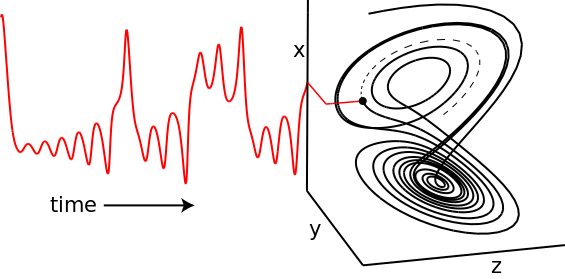
\includegraphics[width=250px]{Lorenz_Projection} 

}

\caption{Time Series Projection from the Lorenz Attractor.}\label{fig:LorenzProjection}
\end{figure}

Although different time series observed from a system can represent
independent state variables, in general, each time series is an
\emph{observation function} of the system state that may convolve
several different state variables.

\hypertarget{attractor-reconstruction-takens-theorem}{%
\subsection{Attractor Reconstruction / Takens'
Theorem}\label{attractor-reconstruction-takens-theorem}}

The goal of EDM is to reconstruct the system dynamics from time series
data. As seen above, a time series can be thought of as sequential
projections of the motion on an attractor; in other words, information
about the behavior is encoded in the temporal ordering of the time
series. Takens' Theorem (Takens 1981) states that mathematically valid
and property preserving reconstructions of the attractor can be created
using lags of a single time series, then substituting those lagged time
series for unknown or unobserved variables. In other words, instead of
representing the system state using a complete set of state variables,
we can instead use an \texttt{E}-dimensional lagged-coordinate
embedding:

\[ \vec{x}_t = \langle x_t, x_{t-\tau}, \dots, x_{t-(E-1)\tau} \rangle \]

\begin{figure}[h]

{\centering 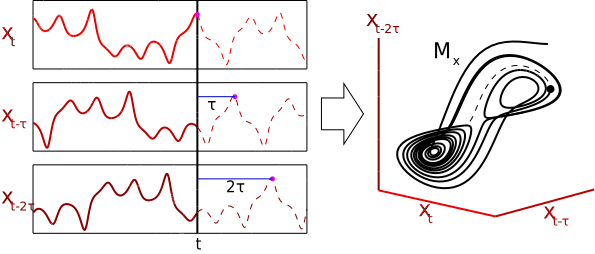
\includegraphics[width=250px]{Lorenz_Reconstruct} 

}

\caption{Attractor Reconstruction from 3 Lagged Coordinates}\label{fig:fig_attractor_reconstruction}
\end{figure}

If sufficient lags are used, the reconstruction preserves essential
mathematical properties of the original system: reconstructed states
will map one-to-one to actual system states, and nearby points in the
reconstruction will correspond to similar system states. Figure 2 shows
a reconstruction of the Lorenz attractor where the reconstructed system
state is comprised of 3 lags of variable \(x\). Here, the visual
similarity between the reconstruction and the original Lorenz Attractor
is quite clear.

As a consequence of the fact that dynamical properties of the original
system can be recovered from a single time series, there are multiple
applications. For example, empirical models can be used for forecasting
(Sugihara and May 1990), to understand nonlinear behavior (Sugihara
1994), or to uncover mechanism (Dixon, Milicich, and Sugihara 1999).
Moreover, recent work describes how EDM can be used to identify causal
interactions, by testing whether two time series are observed from the
same system (Sugihara et al. 2012). In the next section, we demonstrate
how \textbf{rEDM} can be used to accomplish these various tasks.

\hypertarget{demonstration-of-edm}{%
\section{Demonstration of EDM}\label{demonstration-of-edm}}

\hypertarget{nearest-neighbor-forecasting-using-simplex-projection}{%
\subsection{Nearest Neighbor Forecasting using Simplex
Projection}\label{nearest-neighbor-forecasting-using-simplex-projection}}

As mentioned previously, the reconstruction will map one-to-one to the
original attractor manifold if enough lags are used (i.e.~if the
reconstruction has a sufficiently large embedding dimension). If the
embedding dimension is too small, then reconstructed states can overlap
and appear to be the same even though they actually correspond to
different states. These ``singularities'' will result in poor forecast
performance because the system behavior cannot be uniquely determined in
the reconstruction. As a consequence, we can use prediction skill as an
indicator for identifying the optimal embedding dimension. In the
following example we demonstrate the \texttt{Simplex()} projection
nearest neighbor forecasting method (Sugihara and May 1990), and its'
extension \texttt{EmbedDimension()} that automates evaluation of an
optimal embedding dimension.

\hypertarget{example}{%
\subsubsection{Example}\label{example}}

In this example, time series come from a simulation of the tent map that
exhibits chaotic behavior. The tent map is a discrete-time dynamic
system, where a sequence, \(x_t\), on the interval \([0, 1]\) is
iterated according to:

\begin{equation*}
  x_{t+1} = \begin{cases}
            2x_t     & x_t <   \frac{1}{2}\\
            2(1-x_t) & x_t \ge \frac{1}{2}
            \end{cases}
\end{equation*}

In \textbf{rEDM}, a sample time series of first-differenced values can
be found in dataset \texttt{TentMap}.

We begin by loading the \textbf{rEDM} package and examining the
\texttt{TentMap} data:

\begin{Shaded}
\begin{Highlighting}[]
\KeywordTok{library}\NormalTok{(rEDM)}
\KeywordTok{str}\NormalTok{(TentMap)}
\end{Highlighting}
\end{Shaded}

\begin{verbatim}
## 'data.frame':    999 obs. of  2 variables:
##  $ Time   : int  1 2 3 4 5 6 7 8 9 10 ...
##  $ TentMap: num  -0.0992 -0.6013 0.7998 -0.7944 0.798 ...
\end{verbatim}

We can see that the data consists of a data.frame with two columns:
\texttt{Time} and \texttt{TentMap}. All rEDM input data files or
data.frames are assumed to have a time vector in the first column. Data
files are expected to be in .csv format with the first line a header of
column names, data.frames are also expected to have column names.

The \texttt{Simplex} function has 5 required parameters:

\begin{longtable}[]{@{}llll@{}}
\toprule
\endhead
1. & \texttt{columns} & \texttt{TentMap} & name of column(s) of
embedding library\tabularnewline
2. & \texttt{target} & \texttt{TentMap} & name of column for
prediction\tabularnewline
3. & \texttt{lib} & \texttt{"1\ 100"} & start stop indices of embedding
library\tabularnewline
4. & \texttt{pred} & \texttt{"201\ 500"} & start stop indices of
predictions\tabularnewline
5. & \texttt{E} & \texttt{3} & embedding dimension\tabularnewline
\bottomrule
\end{longtable}

\texttt{columns} specifies the timeseries vector(s) that form the
library, \texttt{target} is the column on which predictions will be
made. \texttt{lib} defines row indices of the ``training'' portion of
data, \texttt{pred} corresponds to row indices of the ``test'' portion,
and \texttt{E} defines the embedding dimension.

\emph{Note that if any overlap in the lib and pred is found, it will
enable leave-one-out cross-validation. If \texttt{verbose\ =\ TRUE}, a
warning message will be raised.}

In this univariate case, we specify the ``TentMap'' column of the data
frame for both \texttt{columns} and \texttt{target}, and select the
first 100 points (indices 1 to 100) in the time series to constitute the
``library set'', and a separate 300 point span (indices 201 to 500) as
the ``prediction set''.

Default parameters of \texttt{knn} (k-nearest neighbors) and \texttt{Tp}
(time-to-prediction) are assumed. The default \texttt{knn\ =\ 0} sets
the number of nearest neighbors to \texttt{E\ +\ 1}, and default
\texttt{Tp} is 1 timestep (observation row). With these parameters we
demonstrate the \texttt{Simplex()} function:

\begin{Shaded}
\begin{Highlighting}[]
\NormalTok{simplex_out <-}\StringTok{ }\KeywordTok{Simplex}\NormalTok{(}\DataTypeTok{dataFrame =}\NormalTok{ TentMap, }\DataTypeTok{lib =} \StringTok{"1 100"}\NormalTok{, }\DataTypeTok{pred =} \StringTok{"201 500"}\NormalTok{, }\DataTypeTok{columns =} \StringTok{"TentMap"}\NormalTok{, }
    \DataTypeTok{target =} \StringTok{"TentMap"}\NormalTok{, }\DataTypeTok{E =} \DecValTok{3}\NormalTok{)}
\NormalTok{simplex_out[}\KeywordTok{c}\NormalTok{(}\DecValTok{1}\OperatorTok{:}\DecValTok{2}\NormalTok{, }\DecValTok{300}\OperatorTok{:}\DecValTok{301}\NormalTok{), ]}
\end{Highlighting}
\end{Shaded}

\begin{verbatim}
##     Time Observations Predictions Pred_Variance
## 1    201         0.94         NaN           NaN
## 2    202         0.11       0.077       0.00015
## 300  500        -1.09      -1.084       0.06366
## 301  501         0.91       0.873       0.00255
\end{verbatim}

Note that the returned data.frame has 1 \texttt{NaN} as the first
\texttt{Predictions} point since \texttt{Tp\ =\ 1}, and, the last
\texttt{Observations} will likewise be \texttt{NaN} with the time vector
adjusted to accommodate \texttt{Tp} rows beyond the data as needed.

Computation of Pearson correlation, MAE and RMSE errors between the
forecast \texttt{Observations} and \texttt{Predictions} can be performed
with the \texttt{ComputeError()} function.

\begin{Shaded}
\begin{Highlighting}[]
\KeywordTok{ComputeError}\NormalTok{(simplex_out}\OperatorTok{$}\NormalTok{Observations, simplex_out}\OperatorTok{$}\NormalTok{Predictions)}
\end{Highlighting}
\end{Shaded}

\begin{verbatim}
## $MAE
## [1] 0.14
## 
## $rho
## [1] 0.94
## 
## $RMSE
## [1] 0.23
\end{verbatim}

\hypertarget{optimal-embedding-dimension}{%
\subsection{Optimal embedding
dimension}\label{optimal-embedding-dimension}}

As noted earlier, identification of the optimal embedding dimension to
best ``unfold'' the dynamics can be assessed with simplex prediction
skill. \textbf{rEDM} provides the \texttt{EmbedDimension()} function to
automate this task. \texttt{EmbedDimension()} parallelises function
calls to \texttt{Simplex()}, which automatically sets values of
\texttt{E} from 1 to \texttt{maxE}=10. Continuing with the previous
example, we invoke \texttt{EmbedDimension()}:

\begin{Shaded}
\begin{Highlighting}[]
\NormalTok{rho_E <-}\StringTok{ }\KeywordTok{EmbedDimension}\NormalTok{(}\DataTypeTok{dataFrame =}\NormalTok{ TentMap, }\DataTypeTok{lib =} \StringTok{"1 100"}\NormalTok{, }\DataTypeTok{pred =} \StringTok{"201 500"}\NormalTok{, }\DataTypeTok{columns =} \StringTok{"TentMap"}\NormalTok{, }
    \DataTypeTok{target =} \StringTok{"TentMap"}\NormalTok{)}
\end{Highlighting}
\end{Shaded}

\begin{figure}[h]

{\centering \includegraphics{rEDM-tutorial_files/figure-latex/Embed_Dim_TentMap-1} 

}

\caption{TentMap data prediction skill vs. embedding dimension.}\label{fig:Embed_Dim_TentMap}
\end{figure}

The output is a data.frame with columns \texttt{E} and \texttt{rho}
detailing the embedding dimension and Pearson correlation coefficient
between the simplex projected forecast at \texttt{Tp\ =\ 1} timesteps
ahead, and the observed data over the \texttt{pred} indices. Here, we
observe that forecast skill peaks at \texttt{E\ =\ 2}, indicating that
the dynamics of our data are unfolded best in 2 dimensions. \emph{Note
that this optimal value does not have to correspond to the
dimensionality of the original system.} The forecast skill will be
affected by factors such as observational noise, process error, and time
series length, and so it is more useful to think of the embedding
dimension as a practical measure that is dependent on properties of the
data.

\hypertarget{prediction-decay}{%
\subsection{Prediction Decay}\label{prediction-decay}}

An important property of many natural systems is that nearby
trajectories eventually diverge over time (i.e.~``deterministic chaos''
-- the ``butterfly effect''). In essence, this means that while
short-term prediction is often possible, information about the
predictive state of the system is diluted over time, hindering long-term
forecasting. We can demonstrate this effect by examining how prediction
skill changes as we increase the \texttt{Tp} argument, the ``time to
prediction'', defining the number of time steps into the future at which
forecasts are made. \textbf{rEDM} provides the
\texttt{PredictInterval()} function to automate this task.

\hypertarget{example-1}{%
\subsubsection{Example}\label{example-1}}

Using the same data with the \texttt{PredictInterval()} function, we
supply the embedding dimension parameter with the value determined
previously (\texttt{E\ =\ 2}):

\begin{Shaded}
\begin{Highlighting}[]
\NormalTok{rho_Tp <-}\StringTok{ }\KeywordTok{PredictInterval}\NormalTok{(}\DataTypeTok{dataFrame =}\NormalTok{ TentMap, }\DataTypeTok{lib =} \StringTok{"1 100"}\NormalTok{, }\DataTypeTok{pred =} \StringTok{"201 500"}\NormalTok{, }\DataTypeTok{target =} \StringTok{"TentMap"}\NormalTok{, }
    \DataTypeTok{columns =} \StringTok{"TentMap"}\NormalTok{, }\DataTypeTok{E =} \DecValTok{2}\NormalTok{)}
\end{Highlighting}
\end{Shaded}

\begin{figure}[h]

{\centering \includegraphics{rEDM-tutorial_files/figure-latex/Prediction_interval_on_TentMap-1} 

}

\caption{Tent map first differences simplex prediction skill as a function of forecast interval.}\label{fig:Prediction_interval_on_TentMap}
\end{figure}

As above, the returned object is a data.frame with forecast skill
\texttt{rho} and time to prediction \texttt{Tp}. As expected (because
the parameters chosen for the tent map fall in the region for chaotic
behavior), the decline in forecast skill (\texttt{rho}
\(\rightarrow 0\)) as the forecast interval \texttt{Tp} increases,
indicates that the system may be chaotic.

\hypertarget{identifying-nonlinearity}{%
\subsection{Identifying Nonlinearity}\label{identifying-nonlinearity}}

One concern is that time series may show predictability even if they are
purely stochastic, they behave similarly to autocorrelated red noise.
Fortunately, we can distinguish between red noise and nonlinear
deterministic behavior by using S-maps as described in (Sugihara 1994).

In contrast to the nearest-neighbor interpolation of simplex projection,
the S-map forecasting method (Sugihara 1994) fits local linear maps to
describe the dynamics. In addition to the standard set of parameters for
a lagged-coordinate reconstruction as in simplex, S-maps contain a
nonlinear localisation parameter, \(\theta\), that determines the degree
to which points are weighted when fitting the local linear map. For
example, when \(\theta = 0\), all points are equally weighted, such that
the local linear map is identical for different points in the
reconstructed state-space. As such, the S-map will be identical to a
global linear map (i.e.~an autoregressive model). When values of
\(\theta\) are greater than \(0\), nearby points in the state space
receive larger weight, and the local linear map can vary in state-space
to accommodate nonlinear behavior.

Consequently, if the time series are sampled from autoregressive red
noise, then the linear model (\(\theta = 0\)) should produce better
forecasts, because the global linear map (which will, in effect, be
fitted to more data points) will reduce the effects of observation error
compared to local linear maps. In contrast, if forecast skill increases
for \(\theta > 0\), then the results are suggestive of nonlinear
dynamics wherein better forecasts are achieved when the local linear map
can change depending on the location in state-space: it is a better
description of state-dependent behavior.

\hypertarget{example-2}{%
\subsubsection{Example}\label{example-2}}

The \texttt{PredictNonlinear()} function provides an evaluation of S-map
forecast skill as a function of the localisation parameter
\texttt{theta}. If unspecified, \texttt{theta} values will range from
0.01 to 9.

Typically, when using \texttt{S-map} to test for nonlinear behavior, we
want to use all available points in the reconstruction of the local
linear map, not just \texttt{knn} nearest neighbors as in simplex
projection. With all points available, S-map uses the \texttt{theta}
parameter to control the weighting assigned to individual points,
thereby localising the dynamics to capture nonlinear behavior. When
\texttt{knn\ =\ 0}, the default, \texttt{SMap()} will use all available
points.

Here we use an embedding dimension of \texttt{E\ =\ 2} and the same
parameters as in the previous examples, however, we specify the
``TentMapNoise'' data that adds Gaussian noise to the TentMap data as
one would normally encounter with noisy observational data.

\begin{Shaded}
\begin{Highlighting}[]
\NormalTok{rho_theta <-}\StringTok{ }\KeywordTok{PredictNonlinear}\NormalTok{(}\DataTypeTok{dataFrame =}\NormalTok{ TentMapNoise, }\DataTypeTok{lib =} \StringTok{"1 100"}\NormalTok{, }\DataTypeTok{pred =} \StringTok{"201 500"}\NormalTok{, }
    \DataTypeTok{target =} \StringTok{"TentMap"}\NormalTok{, }\DataTypeTok{columns =} \StringTok{"TentMap"}\NormalTok{, }\DataTypeTok{E =} \DecValTok{2}\NormalTok{)}
\end{Highlighting}
\end{Shaded}

\begin{figure}[h]

{\centering \includegraphics{rEDM-tutorial_files/figure-latex/Predict_nonlinear_on_TentMap-1} 

}

\caption{Tent map first differences S-map prediction skill as a function of S-map localisation parameter.}\label{fig:Predict_nonlinear_on_TentMap}
\end{figure}

The result is a data.frame with columns \texttt{Theta} and \texttt{rho}.
Here, we see that forecast skill substantially improves as
\texttt{theta} increases, indicating the presence of nonlinear dynamics.
We also observe a degradation in forecast skill at high values of
\texttt{theta} as the local linear map overfits to insufficient nearest
neighbors.

\hypertarget{simplex-and-smap-functions}{%
\subsection{\texorpdfstring{\texttt{Simplex()} and \texttt{SMap()}
functions}{Simplex() and SMap() functions}}\label{simplex-and-smap-functions}}

The functions \texttt{EmbedDimension()}, \texttt{PredictInterval()} and
\texttt{PredictNonlinear()} are multithreaded wrapper functions for the
\texttt{Simplex()} and \texttt{SMap()} algorithms.
\texttt{EmbedDimension()} and \texttt{PredictInterval()} parallelise
calls to \texttt{Simplex()} to evaluate forecast skill as a function of
embedding dimension and prediction interval respectively.
\texttt{PredictNonlinear()} parallelises calls to \texttt{SMap()} to
assess predictive skill as a function of the nearest neighbor
localisation parameter. However, one can equivalently call the
underlying \texttt{Simplex()} and \texttt{SMap()} functions directly.

\hypertarget{simplex}{%
\subsubsection{\texorpdfstring{\texttt{Simplex()}}{Simplex()}}\label{simplex}}

For example, evaluation of the simplex prediction at an optimal
embedding dimension of \texttt{E\ =\ 2} can be performed as:

\begin{Shaded}
\begin{Highlighting}[]
\NormalTok{tentMapPredict <-}\StringTok{ }\KeywordTok{Simplex}\NormalTok{(}\DataTypeTok{dataFrame =}\NormalTok{ TentMap, }\DataTypeTok{lib =} \StringTok{"1 100"}\NormalTok{, }\DataTypeTok{pred =} \StringTok{"201 500"}\NormalTok{, }\DataTypeTok{target =} \StringTok{"TentMap"}\NormalTok{, }
    \DataTypeTok{columns =} \StringTok{"TentMap"}\NormalTok{, }\DataTypeTok{E =} \DecValTok{2}\NormalTok{)}

\KeywordTok{ComputeError}\NormalTok{(tentMapPredict}\OperatorTok{$}\NormalTok{Observations, tentMapPredict}\OperatorTok{$}\NormalTok{Predictions)}\OperatorTok{$}\NormalTok{rho}
\end{Highlighting}
\end{Shaded}

\begin{verbatim}
## [1] 0.96
\end{verbatim}

\hypertarget{smap}{%
\subsubsection{\texorpdfstring{\texttt{SMap()}}{SMap()}}\label{smap}}

An individual S-map evaluation corresponding to the optimal
\texttt{PredictNonlinear()} result from above is:

\begin{Shaded}
\begin{Highlighting}[]
\NormalTok{smap =}\StringTok{ }\KeywordTok{SMap}\NormalTok{(}\DataTypeTok{dataFrame =}\NormalTok{ TentMapNoise, }\DataTypeTok{lib =} \StringTok{"1 100"}\NormalTok{, }\DataTypeTok{pred =} \StringTok{"201 500"}\NormalTok{, }\DataTypeTok{target =} \StringTok{"TentMap"}\NormalTok{, }
    \DataTypeTok{columns =} \StringTok{"TentMap"}\NormalTok{, }\DataTypeTok{E =} \DecValTok{2}\NormalTok{, }\DataTypeTok{theta =} \DecValTok{3}\NormalTok{)}
\end{Highlighting}
\end{Shaded}

\texttt{SMap()} returns a named list with \texttt{predictions} and
\texttt{coefficients} data.frames, with \texttt{NaN} inserted
appropriately where no predictions or observations are available.

\begin{Shaded}
\begin{Highlighting}[]
\KeywordTok{head}\NormalTok{(}\KeywordTok{cbind}\NormalTok{(smap}\OperatorTok{$}\NormalTok{predictions, smap}\OperatorTok{$}\NormalTok{coefficients), }\DecValTok{2}\NormalTok{)}
\end{Highlighting}
\end{Shaded}

\begin{verbatim}
##   Time Observations Predictions Pred_Variance Time   C0 ∂TentMap(t-0)/∂TentMap
## 1  201         0.99         NaN           NaN  201  NaN                    NaN
## 2  202         0.16       -0.14          0.28  202 -1.1                  -0.33
##   ∂TentMap(t-1)/∂TentMap
## 1                    NaN
## 2                   -1.1
\end{verbatim}

\begin{Shaded}
\begin{Highlighting}[]
\KeywordTok{tail}\NormalTok{(}\KeywordTok{cbind}\NormalTok{(smap}\OperatorTok{$}\NormalTok{predictions, smap}\OperatorTok{$}\NormalTok{coefficients), }\DecValTok{2}\NormalTok{)}
\end{Highlighting}
\end{Shaded}

\begin{verbatim}
##     Time Observations Predictions Pred_Variance Time    C0
## 300  500         -1.3       -0.63          0.36  500 -0.33
## 301  501          1.1        0.92          0.41  501  0.24
##     ∂TentMap(t-0)/∂TentMap ∂TentMap(t-1)/∂TentMap
## 300                  -0.78                  -0.16
## 301                  -0.52                  -0.03
\end{verbatim}

\hypertarget{generalized-takens-theorem}{%
\subsection{Generalized Takens
Theorem}\label{generalized-takens-theorem}}

A practical reality is that sampled observations of complex dynamics are
usually composed of finite, noisy data. Additionally, the presence of
stochastic, non-deterministic drivers means that ``multivariate''
reconstructions can often be a better description than ``univariate''
reconstructions. This means that in addition to creating an attractor
from lags of one time series, it can be advantageous to combine
different time series to create the phase-space embedding, provided they
are all observed from the same system (Sauer, Yorke, and Casdagli 1991;
Deyle and Sugihara 2011).

In \textbf{rEDM}, the \texttt{Simplex()} and \texttt{SMap()} functions
allow multivariate reconstructions from any set of observation vectors.
A multivariate reconstruction is defined by specifying which columns to
use as coordinates in the \texttt{columns} argument, and which column is
to be forecast in the \texttt{target} argument. By default,
\textbf{rEDM} will create Takens time-delay embeddings from univariate
or multivariate data, however, this can be prevented by setting the
\texttt{embedded} parameter \texttt{TRUE}. In this case, the input data
are assumed to already constitute a valid multidimensional embedding,
and no time-delay embedding is performed.

\hypertarget{example-3}{%
\subsubsection{Example}\label{example-3}}

We begin by examining an example dataset from a coupled 3-species model
system.

\begin{Shaded}
\begin{Highlighting}[]
\KeywordTok{head}\NormalTok{(block_3sp, }\DecValTok{3}\NormalTok{)}
\end{Highlighting}
\end{Shaded}

\begin{verbatim}
##   time   x_t x_t-1 x_t-2   y_t y_t-1 y_t-2  z_t z_t-1 z_t-2
## 1    3 -1.92  1.24 -0.74 -0.11  1.49 -1.27  1.5 -0.48 -1.86
## 2    4 -0.96 -1.92  1.24 -1.11 -0.11  1.49 -1.5  1.54 -0.48
## 3    5  1.33 -0.96 -1.92  2.39 -1.11 -0.11 -1.1 -1.49  1.54
\end{verbatim}

Here, \texttt{block\_3sp} is a 10-column data.frame with 9 data columns.
This data has already been time-delay embedded to dimension
\texttt{E\ =\ 3} with a time delay of \texttt{tau\ =\ -1}. We use
simplex forecasting based on a multivariate embedding of the three data
vectors \texttt{x\_t\ x\_t-1\ z\_t} with \texttt{embedded\ =\ TRUE} and
\texttt{E\ =\ 3}:

\begin{Shaded}
\begin{Highlighting}[]
\NormalTok{smplx_3species =}\StringTok{ }\KeywordTok{Simplex}\NormalTok{(}\DataTypeTok{dataFrame =}\NormalTok{ block_3sp, }\DataTypeTok{lib =} \StringTok{"1 100"}\NormalTok{, }\DataTypeTok{pred =} \StringTok{"101 190"}\NormalTok{, }
    \DataTypeTok{E =} \DecValTok{3}\NormalTok{, }\DataTypeTok{columns =} \StringTok{"x_t x_t-1 z_t"}\NormalTok{, }\DataTypeTok{target =} \StringTok{"x_t"}\NormalTok{, }\DataTypeTok{embedded =} \OtherTok{TRUE}\NormalTok{)}
\end{Highlighting}
\end{Shaded}

A plot of the predictions vs.~observations can be examined with:

\begin{Shaded}
\begin{Highlighting}[]
\NormalTok{err =}\StringTok{ }\KeywordTok{ComputeError}\NormalTok{(smplx_3species}\OperatorTok{$}\NormalTok{Observations, smplx_3species}\OperatorTok{$}\NormalTok{Predictions)}
\KeywordTok{plot}\NormalTok{(smplx_3species}\OperatorTok{$}\NormalTok{Observations, smplx_3species}\OperatorTok{$}\NormalTok{Predictions, }\DataTypeTok{pch =} \DecValTok{19}\NormalTok{, }\DataTypeTok{cex =} \FloatTok{0.5}\NormalTok{, }
    \DataTypeTok{xlab =} \StringTok{"Observations"}\NormalTok{, }\DataTypeTok{ylab =} \StringTok{"Predictions"}\NormalTok{, }\DataTypeTok{main =} \StringTok{"3 Species x_t"}\NormalTok{)}
\KeywordTok{abline}\NormalTok{(}\DataTypeTok{a =} \DecValTok{0}\NormalTok{, }\DataTypeTok{b =} \DecValTok{1}\NormalTok{, }\DataTypeTok{lty =} \DecValTok{2}\NormalTok{, }\DataTypeTok{col =} \StringTok{"blue"}\NormalTok{)}
\KeywordTok{text}\NormalTok{(}\OperatorTok{-}\DecValTok{1}\NormalTok{, }\DecValTok{1}\NormalTok{, }\KeywordTok{paste}\NormalTok{(}\KeywordTok{capture.output}\NormalTok{(}\KeywordTok{cbind}\NormalTok{(err)), }\DataTypeTok{collapse =} \StringTok{"}\CharTok{\textbackslash{}n}\StringTok{"}\NormalTok{))}
\end{Highlighting}
\end{Shaded}

\begin{figure}[h]

{\centering \includegraphics{rEDM-tutorial_files/figure-latex/plot_3_species-1} 

}

\caption{Scatter plot of simplex forecast of $x_t$ vs. observations.}\label{fig:plot_3_species}
\end{figure}

\hypertarget{s-map-coefficients}{%
\subsection{S-map Coefficients}\label{s-map-coefficients}}

As described in (Deyle et al. 2016), S-map coefficients from the
appropriate multivariate embedding can be interpreted as dynamic,
time-varying interaction strengths. We demonstrate this with a chaotic
timeseries described in (Lorenz 1996), defined for N variables k=1,
\ldots{} N, as

\begin{equation*}
  \frac{ dx_{k} }{ dt } = -X_{k-2} X_{k-1} + X_{k-1} X_{k+1} - X_k + F
\end{equation*}

The \texttt{Lorenz5D} data.frame contains a N=5 dimensional system with
F=8 from (Lorenz 1996). Here, we use \texttt{SMap()} to compute a
4-dimensional forecast at \texttt{Tp}=1:

\begin{Shaded}
\begin{Highlighting}[]
\NormalTok{smap_Lorenz <-}\StringTok{ }\KeywordTok{SMap}\NormalTok{(}\DataTypeTok{dataFrame =}\NormalTok{ Lorenz5D, }\DataTypeTok{lib =} \StringTok{"1 500"}\NormalTok{, }\DataTypeTok{pred =} \StringTok{"601 900"}\NormalTok{, }\DataTypeTok{E =} \DecValTok{4}\NormalTok{, }
    \DataTypeTok{theta =} \DecValTok{3}\NormalTok{, }\DataTypeTok{columns =} \StringTok{"V1 V2 V3 V4"}\NormalTok{, }\DataTypeTok{target =} \StringTok{"V1"}\NormalTok{, }\DataTypeTok{embedded =} \OtherTok{TRUE}\NormalTok{)}
\end{Highlighting}
\end{Shaded}

As noted earlier, \texttt{SMap()} returns a named list with two data
frames, \texttt{predictions} and \texttt{coefficients}:

\begin{Shaded}
\begin{Highlighting}[]
\KeywordTok{head}\NormalTok{(}\KeywordTok{cbind}\NormalTok{(smap_Lorenz}\OperatorTok{$}\NormalTok{predictions, smap_Lorenz}\OperatorTok{$}\NormalTok{coefficients[, }\DecValTok{2}\OperatorTok{:}\DecValTok{6}\NormalTok{]), }\DecValTok{3}\NormalTok{)}
\end{Highlighting}
\end{Shaded}

\begin{verbatim}
##    Time Observations Predictions Pred_Variance      C0 ∂V1/∂V1 ∂V2/∂V1
## 1 40.00        3.485         NaN           NaN     NaN     NaN     NaN
## 2 40.05        4.214       4.123         8.197 -0.4830  0.9914  0.1313
## 3 40.10        4.849       4.744         8.947 -0.5544  0.9890  0.1530
##     ∂V3/∂V1 ∂V4/∂V1
## 1       NaN     NaN
## 2 -0.011692 0.04222
## 3 -0.006055 0.02284
\end{verbatim}

Here, we plot the time series for the observed (blue) and predicted
(red) values of \texttt{V1} in the top panel; and the inferred
interactions (S-map coefficients) for the influence of \texttt{V4},
\texttt{V3} and \texttt{V2} on future values of \texttt{V1} in the lower
panels.

\begin{Shaded}
\begin{Highlighting}[]
\NormalTok{predictions =}\StringTok{ }\NormalTok{smap_Lorenz}\OperatorTok{$}\NormalTok{predictions}
\NormalTok{coefficients =}\StringTok{ }\NormalTok{smap_Lorenz}\OperatorTok{$}\NormalTok{coefficients}
\NormalTok{Time =}\StringTok{ }\NormalTok{predictions}\OperatorTok{$}\NormalTok{Time}

\KeywordTok{plot}\NormalTok{(Time, predictions}\OperatorTok{$}\NormalTok{Observations, }\DataTypeTok{type =} \StringTok{"l"}\NormalTok{, }\DataTypeTok{col =} \StringTok{"blue"}\NormalTok{, }\DataTypeTok{ylab =} \StringTok{"V1"}\NormalTok{, }\DataTypeTok{xlab =} \StringTok{""}\NormalTok{, }
    \DataTypeTok{lwd =} \DecValTok{2}\NormalTok{, }\DataTypeTok{cex.lab =} \FloatTok{1.3}\NormalTok{, }\DataTypeTok{cex.axis =} \FloatTok{1.3}\NormalTok{)}
\KeywordTok{lines}\NormalTok{(Time, predictions}\OperatorTok{$}\NormalTok{Predictions, }\DataTypeTok{lwd =} \DecValTok{2}\NormalTok{, }\DataTypeTok{col =} \StringTok{"red"}\NormalTok{)}
\KeywordTok{legend}\NormalTok{(}\StringTok{"topright"}\NormalTok{, }\DataTypeTok{legend =} \KeywordTok{c}\NormalTok{(}\StringTok{"observed"}\NormalTok{, }\StringTok{"predicted"}\NormalTok{), }\DataTypeTok{fill =} \KeywordTok{c}\NormalTok{(}\StringTok{"blue"}\NormalTok{, }\StringTok{"red"}\NormalTok{), }
    \DataTypeTok{bty =} \StringTok{"n"}\NormalTok{, }\DataTypeTok{cex =} \FloatTok{1.3}\NormalTok{)}

\KeywordTok{plot}\NormalTok{(Time, coefficients[, }\DecValTok{6}\NormalTok{], }\DataTypeTok{type =} \StringTok{"l"}\NormalTok{, }\DataTypeTok{col =} \StringTok{"brown"}\NormalTok{, }\DataTypeTok{ylab =} \StringTok{"∂V4/∂V1"}\NormalTok{, }\DataTypeTok{xlab =} \StringTok{""}\NormalTok{, }
    \DataTypeTok{lwd =} \DecValTok{2}\NormalTok{, }\DataTypeTok{cex.lab =} \FloatTok{1.3}\NormalTok{, }\DataTypeTok{cex.axis =} \FloatTok{1.3}\NormalTok{)}
\KeywordTok{plot}\NormalTok{(Time, coefficients[, }\DecValTok{5}\NormalTok{], }\DataTypeTok{type =} \StringTok{"l"}\NormalTok{, }\DataTypeTok{col =} \StringTok{"darkgreen"}\NormalTok{, }\DataTypeTok{ylab =} \StringTok{"∂V3/∂V1"}\NormalTok{, }
    \DataTypeTok{xlab =} \StringTok{""}\NormalTok{, }\DataTypeTok{lwd =} \DecValTok{2}\NormalTok{, }\DataTypeTok{cex.lab =} \FloatTok{1.3}\NormalTok{, }\DataTypeTok{cex.axis =} \FloatTok{1.3}\NormalTok{)}
\KeywordTok{plot}\NormalTok{(Time, coefficients[, }\DecValTok{4}\NormalTok{], }\DataTypeTok{type =} \StringTok{"l"}\NormalTok{, }\DataTypeTok{col =} \StringTok{"blue"}\NormalTok{, }\DataTypeTok{ylab =} \StringTok{"∂V2/∂V1"}\NormalTok{, }\DataTypeTok{xlab =} \StringTok{""}\NormalTok{, }
    \DataTypeTok{lwd =} \DecValTok{2}\NormalTok{, }\DataTypeTok{cex.lab =} \FloatTok{1.3}\NormalTok{, }\DataTypeTok{cex.axis =} \FloatTok{1.3}\NormalTok{)}
\end{Highlighting}
\end{Shaded}

\begin{figure}[h]

{\centering \includegraphics[width=300px]{rEDM-tutorial_files/figure-latex/smap_Lorenz_plot-1} 

}

\caption{S-map prediction and coefficients of Lorenz'96 5-D system.}\label{fig:smap_Lorenz_plot}
\end{figure}

\newpage

\hypertarget{multiview-embedding}{%
\subsection{Multiview Embedding}\label{multiview-embedding}}

The generality of Takens Theorem means that in situations with
multivariate time series, there can often be many different, valid
attractor reconstructions. As described in (Ye and Sugihara 2016),
combining these different models can result in improved forecasts.

Here, we demonstrate this idea using the \texttt{Multiview()} function
with the 3-species data used above. \texttt{Multiview()} operates by
constructing all possible embeddings of dimension \texttt{E} with lag up
to \texttt{E-1}. These embeddings are ranked by forecast skill
(\texttt{rho}) over the \texttt{lib} portion of the data. The individual
forecasts for the top \texttt{multiview} embeddings are then averaged
together. If \texttt{multiview} is not specified it is set to sqrt(C)
where C is the number of E-dimensional combinations created from all
data vectors.

\begin{Shaded}
\begin{Highlighting}[]
\NormalTok{Mview =}\StringTok{ }\KeywordTok{Multiview}\NormalTok{(}\DataTypeTok{dataFrame =}\NormalTok{ block_3sp, }\DataTypeTok{lib =} \StringTok{"1 100"}\NormalTok{, }\DataTypeTok{pred =} \StringTok{"101 190"}\NormalTok{, }\DataTypeTok{E =} \DecValTok{3}\NormalTok{, }
    \DataTypeTok{columns =} \StringTok{"x_t y_t z_t"}\NormalTok{, }\DataTypeTok{target =} \StringTok{"x_t"}\NormalTok{)}
\end{Highlighting}
\end{Shaded}

\texttt{Multiview()} returns a named list with two data.frames:
\texttt{View}, and \texttt{Predictions}. \texttt{View} lists the various
combinations of data embedding vectors used for the forecasts along with
their prediction statistics. \texttt{Predictions} returns the final
averaged multiview projections.

\begin{Shaded}
\begin{Highlighting}[]
\NormalTok{Mview}\OperatorTok{$}\NormalTok{View[}\KeywordTok{which}\NormalTok{(Mview}\OperatorTok{$}\NormalTok{View}\OperatorTok{$}\NormalTok{rho }\OperatorTok{>}\StringTok{ }\FloatTok{0.91}\NormalTok{), ]}
\end{Highlighting}
\end{Shaded}

\begin{verbatim}
##   col_1 col_2 col_3   name_1   name_2   name_3    rho    MAE   RMSE
## 1     1     2     7 x_t(t-0) x_t(t-1) z_t(t-0) 0.9320 0.2391 0.2996
## 3     1     2     3 x_t(t-0) x_t(t-1) x_t(t-2) 0.9395 0.2221 0.2815
## 7     1     2     8 x_t(t-0) x_t(t-1) z_t(t-1) 0.9215 0.2484 0.3202
\end{verbatim}

\newpage

\hypertarget{causality-inference-and-cross-mapping}{%
\subsection{Causality Inference and Cross
Mapping}\label{causality-inference-and-cross-mapping}}

One of the corollaries to the Generalized Takens Theorem is that it
should be possible to cross predict or cross map between variables that
are observed from the same system. Consider two variables, \(x\) and
\(y\) that interact in a dynamic system. Then the univariate
reconstructions based on \(x\) or \(y\) alone should uniquely identify
the system state and and thus the corresponding value of the other
variable.

\begin{figure}[h]

{\centering 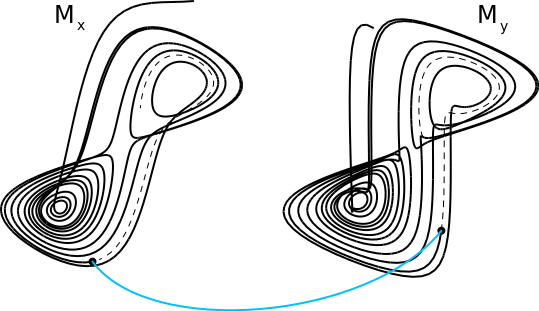
\includegraphics{CrossMap} 

}

\caption{Cross Mapping Between Reconstructions of the Lorenz Attractor}\label{fig:fig_cross_map}
\end{figure}

In the case of unidirectional causality, e.g.~\(x\) causes \(y\), the
causal variable (\(x\)) leaves a signature on the affected variable
(\(y\)). Consequently, the reconstructed states based on \(y\) can be
used to cross predict the values of \(x\) (because the reconstruction
based on \(y\) must be complete, it must include information about the
value of \(x\)). Note that this cross prediction is in the
\emph{opposite} direction of the causal effect. At the same time, cross
prediction from \(x\) to \(y\) will fail, because the time series of
\(x\) behaves independently of \(y\), so a univariate reconstruction
using only lags of \(x\) is necessarily incomplete.

Although \(x\) has incomplete information for predicting \(y\), it does
affect the values of \(y\), and therefore will likely to have nonzero
predictive skill. However, this cross mapping will be limited to the
statistical association between \(x\) and \(y\) and will generally not
improve as longer time series are used for reconstruction. In contrast,
the cross prediction of \(x\) from \(y\) will generally improve. This
convergence is therefore a crucial property for inferring causality. For
practical reasons, the sensitivity of detecting causality this way is
improved if, instead of predicting the future value of another variable,
we estimate the concurrent value of another variable. We refer to this
modified method as cross mapping, because we are not ``predicting'' the
future.

For a more detailed description of using cross mapping to infer
causation, see (Sugihara et al. 2012).

\hypertarget{convergent-cross-mapping-ccm}{%
\subsection{Convergent Cross Mapping
(CCM)}\label{convergent-cross-mapping-ccm}}

In \textbf{rEDM}, convergent cross mapping is implemented as the
\texttt{CCM()} function, which provides a wrapper to compute cross map
skill for different subsamples of the data. In the following example, we
reproduce the analysis from (Sugihara et al. 2012) to identify causality
between anchovy landings in California and Newport Pier sea-surface
temperature. For this example, a previously identified value of
\texttt{3} for the embedding dimension will be used.

To quantify convergence, we compute the cross map skill over many random
subsamples of the time series. The \texttt{libSizes} argument specifies
the size of the library set, and \texttt{sample} specifies the number of
subsamples generated at each library size. \texttt{random} and
\texttt{replacement} specify how the subsamples will be generated. The
default is random sampling without replacement.

\begin{Shaded}
\begin{Highlighting}[]
\NormalTok{cmap <-}\StringTok{ }\KeywordTok{CCM}\NormalTok{(}\DataTypeTok{dataFrame =}\NormalTok{ sardine_anchovy_sst, }\DataTypeTok{E =} \DecValTok{3}\NormalTok{, }\DataTypeTok{Tp =} \DecValTok{0}\NormalTok{, }\DataTypeTok{columns =} \StringTok{"anchovy"}\NormalTok{, }
    \DataTypeTok{target =} \StringTok{"np_sst"}\NormalTok{, }\DataTypeTok{libSizes =} \StringTok{"10 70 5"}\NormalTok{, }\DataTypeTok{sample =} \DecValTok{100}\NormalTok{, }\DataTypeTok{showPlot =} \OtherTok{TRUE}\NormalTok{)}
\end{Highlighting}
\end{Shaded}

\begin{figure}[h]

{\centering \includegraphics{rEDM-tutorial_files/figure-latex/sardine_anchovy_ccm-1} 

}

\caption{Convergent cross mapping of Newport sea surface temperature with anchovy landings.}\label{fig:sardine_anchovy_ccm}
\end{figure}

The output is a data.frame with statistics for each model run (in this
case, 100 models at each library size) as a function of library size.
Recalling that cross mapping indicates causal influence in the reverse
direction (target to source), we see that the cross mapping
\texttt{anchovy:np\_sst} converges at a positive value of \(\rho\),
indicating that Newport sea surface temperature influences anchovy
landings. Because average cross map skill less than 0 means there is no
prediction skill, (predictions should not be anticorrelated with
observations), we infer from the \texttt{np\_sst:anchovy} cross mapping
that anchovy landings do not effect sea surface temperatures.

\hypertarget{real-data-example}{%
\section{Real Data Example}\label{real-data-example}}

\hypertarget{apple-blossom-thrips}{%
\subsection{Apple-Blossom Thrips}\label{apple-blossom-thrips}}

In this example, we use EDM to re-examine the classic apple-blossom
thrips (\emph{Thrips imaginis}) time series from the Wait Institute in
Australia (Davidson and Andrewartha 1948a, 1948b). Seasonal outbreaks of
\emph{Thrips imaginis} were observed to vary greatly in magnitude from
year to year, but large outbreaks tended to coincide across large
spatial domains. This lead to the hypothesis that regional-scale
climatic factors were responsible for controlling the size of the
seasonal outbreaks (what might now be called the Moran effect (Moran
1953)).

\begin{Shaded}
\begin{Highlighting}[]
\KeywordTok{head}\NormalTok{(Thrips, }\DecValTok{2}\NormalTok{)}
\end{Highlighting}
\end{Shaded}

\begin{verbatim}
##   Year Month Thrips_imaginis maxT_degC Rain_mm Season
## 1 1932     4             4.5      19.2   140.1 -0.500
## 2 1932     5            23.4      19.1    53.7 -0.866
\end{verbatim}

The data column \texttt{Thrips\_imaginis} contains counts of
\emph{Thrips imaginis} obtained from the Global Population Dynamics
Database (GPDD) (NERC Centre for Population Biology 2010).
\texttt{maxT\_degC} is the mean maximum daily temperature (\(^\circ\)C)
taken over each month and \texttt{Rain\_mm} is the monthly rainfall
(mm), both from the Waite Institute. The final column \texttt{Season} is
a simple annual sinusoid that peaks in December (the Austral summer) to
emulate an indicator of season.

First, we plot the data. Note that all the time-series variables,
particularly the mean maximum daily temperature, show marked
seasonality.

\begin{figure}[h]

{\centering \includegraphics{rEDM-tutorial_files/figure-latex/thrips plot-1} 

}

\caption{Thrips abundance and environmental variables.}\label{fig:thrips plot}
\end{figure}

\hypertarget{univariate-analysis}{%
\subsubsection{Univariate Analysis}\label{univariate-analysis}}

We first examine the dependence of simplex predictability on the
embedding dimension.

\begin{Shaded}
\begin{Highlighting}[]
\NormalTok{rho_E <-}\StringTok{ }\KeywordTok{EmbedDimension}\NormalTok{(}\DataTypeTok{dataFrame =}\NormalTok{ Thrips, }\DataTypeTok{columns =} \StringTok{"Thrips_imaginis"}\NormalTok{, }\DataTypeTok{target =} \StringTok{"Thrips_imaginis"}\NormalTok{, }
    \DataTypeTok{lib =} \StringTok{"1 72"}\NormalTok{, }\DataTypeTok{pred =} \StringTok{"1 72"}\NormalTok{, }\DataTypeTok{showPlot =} \OtherTok{TRUE}\NormalTok{)}
\end{Highlighting}
\end{Shaded}

\begin{figure}[h]

{\centering \includegraphics{rEDM-tutorial_files/figure-latex/univariate thrips-1} 

}

\caption{Simplex embedding dimension for Thrips abundance.}\label{fig:univariate thrips}
\end{figure}

While there is an initial peak in the simplex prediction at
\texttt{E\ =\ 3}, the global maximum is at \texttt{E\ =\ 8}. This
suggests that both \texttt{E\ =\ 3} and \texttt{E\ =\ 8} are practical
embedding dimensions, although \texttt{E\ =\ 8} is preferrable with a
higher predictive skill.

To test for nonlinearity we use the S-map \texttt{PredictNonlinear()}
function.

\begin{Shaded}
\begin{Highlighting}[]
\NormalTok{E =}\StringTok{ }\DecValTok{8}
\NormalTok{rho_theta_e3 =}\StringTok{ }\KeywordTok{PredictNonlinear}\NormalTok{(}\DataTypeTok{dataFrame =}\NormalTok{ Thrips, }\DataTypeTok{columns =} \StringTok{"Thrips_imaginis"}\NormalTok{, }
    \DataTypeTok{target =} \StringTok{"Thrips_imaginis"}\NormalTok{, }\DataTypeTok{lib =} \StringTok{"1 73"}\NormalTok{, }\DataTypeTok{pred =} \StringTok{"1 73"}\NormalTok{, }\DataTypeTok{E =}\NormalTok{ E)}
\end{Highlighting}
\end{Shaded}

\begin{figure}[h]

{\centering \includegraphics{rEDM-tutorial_files/figure-latex/smap for thrips-1} 

}

\caption{SMap localisation parameter for Thrips abundance.}\label{fig:smap for thrips}
\end{figure}

The S-map results demonstrate clear nonlinearity in the Thrips time
series, as nonlinear models \texttt{theta\ \textgreater{}\ 0} give
substantially better predictions than the linear model
\texttt{theta\ =\ 0}. This suggests that \emph{Thrips}, despite the
strong seasonal dynamics, do not simply track the environment passively,
but have some intrinsic dynamics. To look more closely at the issue of
seasonal drivers, however, we turn to convergent cross-mapping (CCM).

\hypertarget{seasonal-drivers}{%
\subsubsection{Seasonal Drivers}\label{seasonal-drivers}}

Recall that there is a two-part criterion for CCM to be a rigorous test
of causality:

\begin{enumerate}
\def\labelenumi{\arabic{enumi}.}
\tightlist
\item
  The cross map prediction skill is statistically significant when using
  the full time series as the library.
\item
  Cross map prediction demonstrates convergence, i.e.~prediction skill
  increases as more of the time series is used for the library and the
  reconstructed attractor becomes more dense.
\end{enumerate}

For an initial summary, we first compute the cross map skill (measured
with Pearsons \(\rho\)) for each variable pair. Note that \texttt{CCM()}
computes the cross map in both ``directions''.

\begin{Shaded}
\begin{Highlighting}[]
\NormalTok{vars =}\StringTok{ }\KeywordTok{colnames}\NormalTok{(Thrips[}\DecValTok{3}\OperatorTok{:}\DecValTok{6}\NormalTok{])}
\NormalTok{var_pairs =}\StringTok{ }\KeywordTok{combn}\NormalTok{(vars, }\DecValTok{2}\NormalTok{)  }\CommentTok{# Combinations of vars, 2 at a time}
\NormalTok{libSize =}\StringTok{ }\KeywordTok{paste}\NormalTok{(}\KeywordTok{NROW}\NormalTok{(Thrips) }\OperatorTok{-}\StringTok{ }\NormalTok{E, }\KeywordTok{NROW}\NormalTok{(Thrips) }\OperatorTok{-}\StringTok{ }\NormalTok{E, }\DecValTok{10}\NormalTok{, }\DataTypeTok{collapse =} \StringTok{" "}\NormalTok{)}
\NormalTok{ccm_matrix =}\StringTok{ }\KeywordTok{array}\NormalTok{(}\OtherTok{NA}\NormalTok{, }\DataTypeTok{dim =} \KeywordTok{c}\NormalTok{(}\KeywordTok{length}\NormalTok{(vars), }\KeywordTok{length}\NormalTok{(vars)), }\DataTypeTok{dimnames =} \KeywordTok{list}\NormalTok{(vars, }
\NormalTok{    vars))}

\ControlFlowTok{for}\NormalTok{ (i }\ControlFlowTok{in} \DecValTok{1}\OperatorTok{:}\KeywordTok{ncol}\NormalTok{(var_pairs)) \{}
\NormalTok{    ccm_out =}\StringTok{ }\KeywordTok{CCM}\NormalTok{(}\DataTypeTok{dataFrame =}\NormalTok{ Thrips, }\DataTypeTok{columns =}\NormalTok{ var_pairs[}\DecValTok{1}\NormalTok{, i], }\DataTypeTok{target =}\NormalTok{ var_pairs[}\DecValTok{2}\NormalTok{, }
\NormalTok{        i], }\DataTypeTok{libSizes =}\NormalTok{ libSize, }\DataTypeTok{Tp =} \DecValTok{0}\NormalTok{, }\DataTypeTok{E =}\NormalTok{ E, }\DataTypeTok{sample =} \DecValTok{100}\NormalTok{)}
    
\NormalTok{    outVars =}\StringTok{ }\KeywordTok{names}\NormalTok{(ccm_out)}
    
\NormalTok{    var_out =}\StringTok{ }\KeywordTok{unlist}\NormalTok{(}\KeywordTok{strsplit}\NormalTok{(outVars[}\DecValTok{2}\NormalTok{], }\StringTok{":"}\NormalTok{))}
\NormalTok{    ccm_matrix[var_out[}\DecValTok{2}\NormalTok{], var_out[}\DecValTok{1}\NormalTok{]] =}\StringTok{ }\NormalTok{ccm_out[}\DecValTok{1}\NormalTok{, }\DecValTok{2}\NormalTok{]}
    
\NormalTok{    var_out =}\StringTok{ }\KeywordTok{unlist}\NormalTok{(}\KeywordTok{strsplit}\NormalTok{(outVars[}\DecValTok{3}\NormalTok{], }\StringTok{":"}\NormalTok{))}
\NormalTok{    ccm_matrix[var_out[}\DecValTok{2}\NormalTok{], var_out[}\DecValTok{1}\NormalTok{]] =}\StringTok{ }\NormalTok{ccm_out[}\DecValTok{1}\NormalTok{, }\DecValTok{3}\NormalTok{]}
\NormalTok{\}}
\end{Highlighting}
\end{Shaded}

We note that \texttt{ccm\_matrix} rows are the second of the
\texttt{CCM()} returned variables, while columns are the first variable.
As outlined earlier, influences are quantified from the \texttt{target}
to the \texttt{columns} variable so that here, rows are considered the
'target\texttt{,\ influencing\ variable,\ and\ columns\ the}columns`
influenced variable.

For comparison we also compute the lagged cross-correlation, allowing
lags of up to \(\pm 6\) months.

\begin{Shaded}
\begin{Highlighting}[]
\NormalTok{corr_matrix <-}\StringTok{ }\KeywordTok{array}\NormalTok{(}\OtherTok{NA}\NormalTok{, }\DataTypeTok{dim =} \KeywordTok{c}\NormalTok{(}\KeywordTok{length}\NormalTok{(vars), }\KeywordTok{length}\NormalTok{(vars)), }\DataTypeTok{dimnames =} \KeywordTok{list}\NormalTok{(vars, }
\NormalTok{    vars))}

\ControlFlowTok{for}\NormalTok{ (ccm_from }\ControlFlowTok{in}\NormalTok{ vars) \{}
    \ControlFlowTok{for}\NormalTok{ (ccm_to }\ControlFlowTok{in}\NormalTok{ vars[vars }\OperatorTok{!=}\StringTok{ }\NormalTok{ccm_from]) \{}
\NormalTok{        ccf_out <-}\StringTok{ }\KeywordTok{ccf}\NormalTok{(Thrips[, ccm_from], Thrips[, ccm_to], }\DataTypeTok{type =} \StringTok{"correlation"}\NormalTok{, }
            \DataTypeTok{lag.max =} \DecValTok{6}\NormalTok{, }\DataTypeTok{plot =} \OtherTok{FALSE}\NormalTok{)}\OperatorTok{$}\NormalTok{acf}
\NormalTok{        corr_matrix[ccm_from, ccm_to] <-}\StringTok{ }\KeywordTok{max}\NormalTok{(}\KeywordTok{abs}\NormalTok{(ccf_out))}
\NormalTok{    \}}
\NormalTok{\}}
\end{Highlighting}
\end{Shaded}

We compare the two matrices.

\begin{Shaded}
\begin{Highlighting}[]
\NormalTok{ccm_matrix}
\end{Highlighting}
\end{Shaded}

\begin{verbatim}
##                 Thrips_imaginis maxT_degC Rain_mm Season
## Thrips_imaginis              NA    0.6055  0.4273 0.5624
## maxT_degC                0.9234        NA  0.8207 0.9625
## Rain_mm                  0.5118    0.4629      NA 0.3930
## Season                   0.9548    0.9918  0.7772     NA
\end{verbatim}

\begin{Shaded}
\begin{Highlighting}[]
\NormalTok{corr_matrix}
\end{Highlighting}
\end{Shaded}

\begin{verbatim}
##                 Thrips_imaginis maxT_degC Rain_mm Season
## Thrips_imaginis              NA    0.4490  0.2668 0.4488
## maxT_degC                0.4490        NA  0.5949 0.9453
## Rain_mm                  0.2668    0.5949      NA 0.5333
## Season                   0.4488    0.9453  0.5333     NA
\end{verbatim}

We can see that the cross map strengths are not symmetric. In general
CCM(X1 : X2) != CCM(X2 : X1). We also notice that the cross map and
correlation between temperature and the seasonal indicator are high,
with the cross map results suggesting that the seasonal variable can
almost perfectly recover the temperature, \(\rho = 0.9918\). This makes
interpretation more complicated, because we have to consider the
possibility that cross mapping is simply identifying the shared
seasonality between two time series. In other words, cross mapping
between temperature and any variable with a seasonal cycle, might
suggest an interaction even if there is no actual causal mechanism.

\hypertarget{convergent-cross-mapping}{%
\paragraph{Convergent Cross-Mapping}\label{convergent-cross-mapping}}

With this in mind, we examine convergence in cross-map predictability,
i.e.~we compute \texttt{rho} as a function of library size \texttt{L}.
The magnitude of the cross-correlation between \emph{Thrips} and the
cross mapped variable is shown as a black dashed line for comparison.

\begin{Shaded}
\begin{Highlighting}[]
\NormalTok{thrips_xmap_maxT <-}\StringTok{ }\KeywordTok{CCM}\NormalTok{(}\DataTypeTok{dataFrame =}\NormalTok{ Thrips, }\DataTypeTok{E =}\NormalTok{ E, }\DataTypeTok{Tp =} \DecValTok{0}\NormalTok{, }\DataTypeTok{columns =} \StringTok{"Thrips_imaginis"}\NormalTok{, }
    \DataTypeTok{target =} \StringTok{"maxT_degC"}\NormalTok{, }\DataTypeTok{libSizes =} \StringTok{"13 73 3"}\NormalTok{, }\DataTypeTok{sample =} \DecValTok{300}\NormalTok{, }\DataTypeTok{showPlot =} \OtherTok{TRUE}\NormalTok{)}
\KeywordTok{abline}\NormalTok{(}\DataTypeTok{h =}\NormalTok{ corr_matrix[}\StringTok{"Thrips_imaginis"}\NormalTok{, }\StringTok{"maxT_degC"}\NormalTok{], }\DataTypeTok{col =} \StringTok{"black"}\NormalTok{, }\DataTypeTok{lty =} \DecValTok{2}\NormalTok{)}

\NormalTok{thrips_xmap_maxT <-}\StringTok{ }\KeywordTok{CCM}\NormalTok{(}\DataTypeTok{dataFrame =}\NormalTok{ Thrips, }\DataTypeTok{E =}\NormalTok{ E, }\DataTypeTok{Tp =} \DecValTok{0}\NormalTok{, }\DataTypeTok{columns =} \StringTok{"Thrips_imaginis"}\NormalTok{, }
    \DataTypeTok{target =} \StringTok{"Rain_mm"}\NormalTok{, }\DataTypeTok{libSizes =} \StringTok{"13 73 3"}\NormalTok{, }\DataTypeTok{sample =} \DecValTok{300}\NormalTok{, }\DataTypeTok{showPlot =} \OtherTok{TRUE}\NormalTok{)}
\KeywordTok{abline}\NormalTok{(}\DataTypeTok{h =}\NormalTok{ corr_matrix[}\StringTok{"Thrips_imaginis"}\NormalTok{, }\StringTok{"Rain_mm"}\NormalTok{], }\DataTypeTok{col =} \StringTok{"black"}\NormalTok{, }\DataTypeTok{lty =} \DecValTok{2}\NormalTok{)}

\NormalTok{thrips_xmap_maxT <-}\StringTok{ }\KeywordTok{CCM}\NormalTok{(}\DataTypeTok{dataFrame =}\NormalTok{ Thrips, }\DataTypeTok{E =}\NormalTok{ E, }\DataTypeTok{Tp =} \DecValTok{0}\NormalTok{, }\DataTypeTok{columns =} \StringTok{"Thrips_imaginis"}\NormalTok{, }
    \DataTypeTok{target =} \StringTok{"Season"}\NormalTok{, }\DataTypeTok{libSizes =} \StringTok{"13 73 3"}\NormalTok{, }\DataTypeTok{sample =} \DecValTok{300}\NormalTok{, }\DataTypeTok{showPlot =} \OtherTok{TRUE}\NormalTok{)}
\KeywordTok{abline}\NormalTok{(}\DataTypeTok{h =}\NormalTok{ corr_matrix[}\StringTok{"Thrips_imaginis"}\NormalTok{, }\StringTok{"Season"}\NormalTok{], }\DataTypeTok{col =} \StringTok{"black"}\NormalTok{, }\DataTypeTok{lty =} \DecValTok{2}\NormalTok{)}
\end{Highlighting}
\end{Shaded}

\begin{figure}[h]

{\centering \includegraphics{rEDM-tutorial_files/figure-latex/ccm thrips-1} 

}

\caption{Thrips cross mapped to climatic variables. Vertical axis is cross map prediction skill (rho).}\label{fig:ccm thrips}
\end{figure}

The results show evidence of convergence for \emph{Thrips} cross mapping
to temperature and season variables, with the \(\rho\) at maximum
library size \texttt{L} significantly exceeding linear correlation. The
rain variable does not indicate a substantially different cross map
interaction, appearing confounded as to causal influence.

In addition, we are still left with the conundrum that temperature and
to a lesser extent, rainfall, are easily predicted from the seasonal
cycle, and so we cannot immediately ignore the possibility that the
cross map results are an artifact of shared seasonal forcing.

To reframe, we wish to reject the null hypothesis that the level of
cross mapping we obtain for \texttt{maxT\_degC} and \texttt{Rain\_mm}
can be solely explained by shared seasonality. This hypothesis can be
tested using randomization tests based on surrogate data. The idea here
is to generate surrogate time series with the same level of shared
seasonality. Cross mapping between the real time series and these
surrogates thus generates a null distribution for \(\rho\), against
which the actual cross map \(\rho\) value can be compared.

\hypertarget{seasonal-surrogate-test}{%
\paragraph{Seasonal Surrogate Test}\label{seasonal-surrogate-test}}

\begin{Shaded}
\begin{Highlighting}[]
\CommentTok{# Create matrix with temperature and rain surrogates (1000 time series vectors)}
\NormalTok{surr_maxT =}\StringTok{ }\KeywordTok{SurrogateData}\NormalTok{(Thrips}\OperatorTok{$}\NormalTok{maxT_degC, }\DataTypeTok{method =} \StringTok{"seasonal"}\NormalTok{, }\DataTypeTok{T_period =} \DecValTok{12}\NormalTok{, }\DataTypeTok{num_surr =} \DecValTok{1000}\NormalTok{, }
    \DataTypeTok{alpha =} \DecValTok{3}\NormalTok{)}
\NormalTok{surr_rain =}\StringTok{ }\KeywordTok{SurrogateData}\NormalTok{(Thrips}\OperatorTok{$}\NormalTok{Rain_mm, }\DataTypeTok{method =} \StringTok{"seasonal"}\NormalTok{, }\DataTypeTok{T_period =} \DecValTok{12}\NormalTok{, }\DataTypeTok{num_surr =} \DecValTok{1000}\NormalTok{, }
    \DataTypeTok{alpha =} \DecValTok{3}\NormalTok{)}

\CommentTok{# Rain cannot be negative}
\NormalTok{surr_rain =}\StringTok{ }\KeywordTok{apply}\NormalTok{(surr_rain, }\DecValTok{2}\NormalTok{, }\ControlFlowTok{function}\NormalTok{(x) \{}
\NormalTok{    i =}\StringTok{ }\KeywordTok{which}\NormalTok{(x }\OperatorTok{<}\StringTok{ }\DecValTok{0}\NormalTok{)}
\NormalTok{    x[i] =}\StringTok{ }\DecValTok{0}
\NormalTok{    x}
\NormalTok{\})}

\CommentTok{# data.frame to hold CCM rho values between Thrips abundance and variable}
\NormalTok{rho_surr <-}\StringTok{ }\KeywordTok{data.frame}\NormalTok{(}\DataTypeTok{maxT =} \KeywordTok{numeric}\NormalTok{(}\DecValTok{1000}\NormalTok{), }\DataTypeTok{Rain =} \KeywordTok{numeric}\NormalTok{(}\DecValTok{1000}\NormalTok{))}

\CommentTok{# data.frames with time, Thrips, and 1000 surrogate climate variables for CCM()}
\NormalTok{maxT_data =}\StringTok{ }\KeywordTok{as.data.frame}\NormalTok{(}\KeywordTok{cbind}\NormalTok{(}\KeywordTok{seq}\NormalTok{(}\DecValTok{1}\OperatorTok{:}\KeywordTok{nrow}\NormalTok{(Thrips)), Thrips}\OperatorTok{$}\NormalTok{Thrips_imaginis, surr_maxT))}
\KeywordTok{names}\NormalTok{(maxT_data) =}\StringTok{ }\KeywordTok{c}\NormalTok{(}\StringTok{"time"}\NormalTok{, }\StringTok{"Thrips_imaginis"}\NormalTok{, }\KeywordTok{paste}\NormalTok{(}\StringTok{"T"}\NormalTok{, }\KeywordTok{as.character}\NormalTok{(}\KeywordTok{seq}\NormalTok{(}\DecValTok{1}\NormalTok{, }\DecValTok{1000}\NormalTok{)), }
    \DataTypeTok{sep =} \StringTok{""}\NormalTok{))}

\NormalTok{rain_data =}\StringTok{ }\KeywordTok{as.data.frame}\NormalTok{(}\KeywordTok{cbind}\NormalTok{(}\KeywordTok{seq}\NormalTok{(}\DecValTok{1}\OperatorTok{:}\KeywordTok{nrow}\NormalTok{(Thrips)), Thrips}\OperatorTok{$}\NormalTok{Thrips_imaginis, surr_rain))}
\KeywordTok{names}\NormalTok{(rain_data) =}\StringTok{ }\KeywordTok{c}\NormalTok{(}\StringTok{"time"}\NormalTok{, }\StringTok{"Thrips_imaginis"}\NormalTok{, }\KeywordTok{paste}\NormalTok{(}\StringTok{"R"}\NormalTok{, }\KeywordTok{as.character}\NormalTok{(}\KeywordTok{seq}\NormalTok{(}\DecValTok{1}\NormalTok{, }\DecValTok{1000}\NormalTok{)), }
    \DataTypeTok{sep =} \StringTok{""}\NormalTok{))}

\CommentTok{# Cross mapping}
\ControlFlowTok{for}\NormalTok{ (i }\ControlFlowTok{in} \DecValTok{1}\OperatorTok{:}\DecValTok{1000}\NormalTok{) \{}
\NormalTok{    targetCol =}\StringTok{ }\KeywordTok{paste}\NormalTok{(}\StringTok{"T"}\NormalTok{, i, }\DataTypeTok{sep =} \StringTok{""}\NormalTok{)  }\CommentTok{# as in maxT_data}
    
\NormalTok{    ccm_out =}\StringTok{ }\KeywordTok{CCM}\NormalTok{(}\DataTypeTok{dataFrame =}\NormalTok{ maxT_data, }\DataTypeTok{E =}\NormalTok{ E, }\DataTypeTok{Tp =} \DecValTok{0}\NormalTok{, }\DataTypeTok{columns =} \StringTok{"Thrips_imaginis"}\NormalTok{, }
        \DataTypeTok{target =}\NormalTok{ targetCol, }\DataTypeTok{libSizes =} \StringTok{"73 73 5"}\NormalTok{, }\DataTypeTok{sample =} \DecValTok{1}\NormalTok{)}
    
\NormalTok{    col =}\StringTok{ }\KeywordTok{paste}\NormalTok{(}\StringTok{"Thrips_imaginis"}\NormalTok{, }\StringTok{":"}\NormalTok{, targetCol, }\DataTypeTok{sep =} \StringTok{""}\NormalTok{)}
    
\NormalTok{    rho_surr}\OperatorTok{$}\NormalTok{maxT[i] =}\StringTok{ }\NormalTok{ccm_out[}\DecValTok{1}\NormalTok{, col]}
\NormalTok{\}}

\ControlFlowTok{for}\NormalTok{ (i }\ControlFlowTok{in} \DecValTok{1}\OperatorTok{:}\DecValTok{1000}\NormalTok{) \{}
\NormalTok{    targetCol =}\StringTok{ }\KeywordTok{paste}\NormalTok{(}\StringTok{"R"}\NormalTok{, i, }\DataTypeTok{sep =} \StringTok{""}\NormalTok{)  }\CommentTok{# as in rain_data}
    
\NormalTok{    ccm_out =}\StringTok{ }\KeywordTok{CCM}\NormalTok{(}\DataTypeTok{dataFrame =}\NormalTok{ rain_data, }\DataTypeTok{E =}\NormalTok{ E, }\DataTypeTok{Tp =} \DecValTok{0}\NormalTok{, }\DataTypeTok{columns =} \StringTok{"Thrips_imaginis"}\NormalTok{, }
        \DataTypeTok{target =}\NormalTok{ targetCol, }\DataTypeTok{libSizes =} \StringTok{"73 73 5"}\NormalTok{, }\DataTypeTok{sample =} \DecValTok{1}\NormalTok{)}
    
\NormalTok{    col =}\StringTok{ }\KeywordTok{paste}\NormalTok{(}\StringTok{"Thrips_imaginis"}\NormalTok{, }\StringTok{":"}\NormalTok{, targetCol, }\DataTypeTok{sep =} \StringTok{""}\NormalTok{)}
    
\NormalTok{    rho_surr}\OperatorTok{$}\NormalTok{Rain[i] =}\StringTok{ }\NormalTok{ccm_out[}\DecValTok{1}\NormalTok{, col]}
\NormalTok{\}}
\end{Highlighting}
\end{Shaded}

We now have a null distribution, and can estimate a \(p\)-value for
rejecting the null hypothesis of mutual seasonality.

\begin{Shaded}
\begin{Highlighting}[]
\DecValTok{1} \OperatorTok{-}\StringTok{ }\KeywordTok{ecdf}\NormalTok{(rho_surr}\OperatorTok{$}\NormalTok{maxT)(ccm_matrix[}\StringTok{"maxT_degC"}\NormalTok{, }\StringTok{"Thrips_imaginis"}\NormalTok{])}
\end{Highlighting}
\end{Shaded}

\begin{verbatim}
## [1] 0
\end{verbatim}

\begin{Shaded}
\begin{Highlighting}[]
\DecValTok{1} \OperatorTok{-}\StringTok{ }\KeywordTok{ecdf}\NormalTok{(rho_surr}\OperatorTok{$}\NormalTok{Rain)(ccm_matrix[}\StringTok{"Rain_mm"}\NormalTok{, }\StringTok{"Thrips_imaginis"}\NormalTok{])}
\end{Highlighting}
\end{Shaded}

\begin{verbatim}
## [1] 0.049
\end{verbatim}

In the case of temperature, the CCM influence we estimated (0.9234) is
higher than the linear correlation (0.449), and is highly significant in
relation to a surrogate null distribution. Regarding rainfall, the CCM
influence (0.5118) is higher than the linear correlate (0.2668), but not
significant at the 95th percentile of the surrogate null distribution.
We note that the original Thrips data collections were at a much higher
frequency than those available through the GPDD, and that monthly
accumulated rainfall may be inadequate to resolve lifecycle influences
on a species with a lifecycle of approximately one month. With more
highly resolved data, it may well be possible to establish significance.

\hypertarget{package-core}{%
\section{Package Core}\label{package-core}}

The \textbf{rEDM} package is implemented as a wrapper to the
\href{github.com/SugiharaLab/cppEDM}{\texttt{cppEDM}} library. All EDM
algorithms are executed in the core \texttt{cppEDM} library and
interfaced through the
\href{cran.r-project.org/web/packages/Rcpp/index.html}{\texttt{Rcpp}}
package.

\hypertarget{data-input}{%
\subsection{Data Input}\label{data-input}}

Data can be input as an R \texttt{data.frame}, or read from a
\texttt{.csv} file. In either case, the first column must define a time
vector, and all columns are expected to be named. The time vector can be
a string encoding a Date, or Datetime format. All subsequent columns are
expected to be numeric.

\hypertarget{s-map-coefficients-and-embedded-data}{%
\subsubsection{S-Map coefficients and embedded
data}\label{s-map-coefficients-and-embedded-data}}

\texttt{SMap()} should be called with a DataFrame that has columns
explicity corresponding to dimensions \texttt{E}. This means that if a
multivariate data set is used, it should not be called with an embedding
from \texttt{Embed()} since \texttt{Embed()} will add lagged coordinates
for each variable. These extra columns will then not correspond to the
intended dimensions in the matrix inversion and prediction
reconstruction and subsequent S-map coefficients. In this case, use the
\texttt{embedded\ =\ TRUE} parameter with the multivariate data so that
columns selected correspond to the proper dimension.

\hypertarget{parameters}{%
\section{Parameters}\label{parameters}}

Since \textbf{rEDM} is a wrapper for the
\href{github.com/SugiharaLab/cppEDM}{\texttt{cppEDM}} library,
parameters largely correspond to function parameters of
\href{github.com/SugiharaLab/cppEDM}{\texttt{cppEDM}}. Primary
parameters are tabulated here.

\begin{longtable}[]{@{}ll@{}}
\toprule
\begin{minipage}[b]{0.09\columnwidth}\raggedright
Parameter\strut
\end{minipage} & \begin{minipage}[b]{0.85\columnwidth}\raggedright
Description\strut
\end{minipage}\tabularnewline
\midrule
\endhead
\begin{minipage}[t]{0.09\columnwidth}\raggedright
pathIn\strut
\end{minipage} & \begin{minipage}[t]{0.85\columnwidth}\raggedright
Filesystem path to input `dataFile'. CSV format.\strut
\end{minipage}\tabularnewline
\begin{minipage}[t]{0.09\columnwidth}\raggedright
dataFile\strut
\end{minipage} & \begin{minipage}[t]{0.85\columnwidth}\raggedright
CSV format data file name. The first column must be a timeindex or time
values.\strut
\end{minipage}\tabularnewline
\begin{minipage}[t]{0.09\columnwidth}\raggedright
\strut
\end{minipage} & \begin{minipage}[t]{0.85\columnwidth}\raggedright
The first row must be column names.\strut
\end{minipage}\tabularnewline
\begin{minipage}[t]{0.09\columnwidth}\raggedright
dataFrame\strut
\end{minipage} & \begin{minipage}[t]{0.85\columnwidth}\raggedright
Input data.frame. The first column must be a time index or time
values.\strut
\end{minipage}\tabularnewline
\begin{minipage}[t]{0.09\columnwidth}\raggedright
\strut
\end{minipage} & \begin{minipage}[t]{0.85\columnwidth}\raggedright
The columns must be named.\strut
\end{minipage}\tabularnewline
\begin{minipage}[t]{0.09\columnwidth}\raggedright
pathOut\strut
\end{minipage} & \begin{minipage}[t]{0.85\columnwidth}\raggedright
Filesystem path for `predictFile' containing output predictions.\strut
\end{minipage}\tabularnewline
\begin{minipage}[t]{0.09\columnwidth}\raggedright
predictFile\strut
\end{minipage} & \begin{minipage}[t]{0.85\columnwidth}\raggedright
Observation and Prediction output file name. CSV format.\strut
\end{minipage}\tabularnewline
\begin{minipage}[t]{0.09\columnwidth}\raggedright
smapFile\strut
\end{minipage} & \begin{minipage}[t]{0.85\columnwidth}\raggedright
Output file containing S-map coefficients.\strut
\end{minipage}\tabularnewline
\begin{minipage}[t]{0.09\columnwidth}\raggedright
lib\strut
\end{minipage} & \begin{minipage}[t]{0.85\columnwidth}\raggedright
String with start and stop indices of input data rows used to create the
library of observations.\strut
\end{minipage}\tabularnewline
\begin{minipage}[t]{0.09\columnwidth}\raggedright
\strut
\end{minipage} & \begin{minipage}[t]{0.85\columnwidth}\raggedright
A single contiguous range is supported.\strut
\end{minipage}\tabularnewline
\begin{minipage}[t]{0.09\columnwidth}\raggedright
pred\strut
\end{minipage} & \begin{minipage}[t]{0.85\columnwidth}\raggedright
String with start and stop indices of input data rows used for
predictions.\strut
\end{minipage}\tabularnewline
\begin{minipage}[t]{0.09\columnwidth}\raggedright
\strut
\end{minipage} & \begin{minipage}[t]{0.85\columnwidth}\raggedright
A single contiguous range is supported.\strut
\end{minipage}\tabularnewline
\begin{minipage}[t]{0.09\columnwidth}\raggedright
D\strut
\end{minipage} & \begin{minipage}[t]{0.85\columnwidth}\raggedright
Multiview dimension.\strut
\end{minipage}\tabularnewline
\begin{minipage}[t]{0.09\columnwidth}\raggedright
E\strut
\end{minipage} & \begin{minipage}[t]{0.85\columnwidth}\raggedright
Embedding dimension.\strut
\end{minipage}\tabularnewline
\begin{minipage}[t]{0.09\columnwidth}\raggedright
Tp\strut
\end{minipage} & \begin{minipage}[t]{0.85\columnwidth}\raggedright
Prediction horizon (number of time column rows).\strut
\end{minipage}\tabularnewline
\begin{minipage}[t]{0.09\columnwidth}\raggedright
knn\strut
\end{minipage} & \begin{minipage}[t]{0.85\columnwidth}\raggedright
Number of nearest neighbors. If knn=0; knn is set to E+1 for Simplex();
set to number of data rows for SMap().\strut
\end{minipage}\tabularnewline
\begin{minipage}[t]{0.09\columnwidth}\raggedright
tau\strut
\end{minipage} & \begin{minipage}[t]{0.85\columnwidth}\raggedright
Lag of time delay embedding specified as number of time column
rows.\strut
\end{minipage}\tabularnewline
\begin{minipage}[t]{0.09\columnwidth}\raggedright
theta\strut
\end{minipage} & \begin{minipage}[t]{0.85\columnwidth}\raggedright
In Smap: S-Map neighbor localisation exponent. Single numeric.\strut
\end{minipage}\tabularnewline
\begin{minipage}[t]{0.09\columnwidth}\raggedright
theta\strut
\end{minipage} & \begin{minipage}[t]{0.85\columnwidth}\raggedright
In PredictNonlinear: A whitespace delimeted string with values of S-map
localisation parameters to be evaluated.\strut
\end{minipage}\tabularnewline
\begin{minipage}[t]{0.09\columnwidth}\raggedright
exclusionRadius\strut
\end{minipage} & \begin{minipage}[t]{0.85\columnwidth}\raggedright
Excludes vectors from the search space of nearest neighbors if their
relative time index is within exclusionRadius.\strut
\end{minipage}\tabularnewline
\begin{minipage}[t]{0.09\columnwidth}\raggedright
columns\strut
\end{minipage} & \begin{minipage}[t]{0.85\columnwidth}\raggedright
String of whitespace separated column name(s) in the input data used to
create the library.\strut
\end{minipage}\tabularnewline
\begin{minipage}[t]{0.09\columnwidth}\raggedright
target\strut
\end{minipage} & \begin{minipage}[t]{0.85\columnwidth}\raggedright
String of column name in the input data used for prediction.\strut
\end{minipage}\tabularnewline
\begin{minipage}[t]{0.09\columnwidth}\raggedright
embedded\strut
\end{minipage} & \begin{minipage}[t]{0.85\columnwidth}\raggedright
Logical specifying if the input data are embedded.\strut
\end{minipage}\tabularnewline
\begin{minipage}[t]{0.09\columnwidth}\raggedright
validLib\strut
\end{minipage} & \begin{minipage}[t]{0.85\columnwidth}\raggedright
Conditional embedding. Boolean vector identifying time series rows to
use in state-space library.\strut
\end{minipage}\tabularnewline
\begin{minipage}[t]{0.09\columnwidth}\raggedright
generateSteps\strut
\end{minipage} & \begin{minipage}[t]{0.85\columnwidth}\raggedright
Generative feedback predictions in Simplex or SMap.\strut
\end{minipage}\tabularnewline
\begin{minipage}[t]{0.09\columnwidth}\raggedright
parameterList\strut
\end{minipage} & \begin{minipage}[t]{0.85\columnwidth}\raggedright
Add parameter dictionary to return objects in Simplex; SMap; CCM;
Multiview.\strut
\end{minipage}\tabularnewline
\begin{minipage}[t]{0.09\columnwidth}\raggedright
libSizes\strut
\end{minipage} & \begin{minipage}[t]{0.85\columnwidth}\raggedright
String of 3 whitespace separated integer values specifying the intial
library size; the final library size; and the library size increment for
CCM.\strut
\end{minipage}\tabularnewline
\begin{minipage}[t]{0.09\columnwidth}\raggedright
sample\strut
\end{minipage} & \begin{minipage}[t]{0.85\columnwidth}\raggedright
Integer specifying the number of random samples to draw at each library
size evaluation for CCM.\strut
\end{minipage}\tabularnewline
\begin{minipage}[t]{0.09\columnwidth}\raggedright
random\strut
\end{minipage} & \begin{minipage}[t]{0.85\columnwidth}\raggedright
Logical to specify random (`TRUE') or sequential library sampling in
CCM.\strut
\end{minipage}\tabularnewline
\begin{minipage}[t]{0.09\columnwidth}\raggedright
replacement\strut
\end{minipage} & \begin{minipage}[t]{0.85\columnwidth}\raggedright
Logical to specify sampling with replacement in CCM.\strut
\end{minipage}\tabularnewline
\begin{minipage}[t]{0.09\columnwidth}\raggedright
includeData\strut
\end{minipage} & \begin{minipage}[t]{0.85\columnwidth}\raggedright
Logical to return all CCM projection data frames.\strut
\end{minipage}\tabularnewline
\begin{minipage}[t]{0.09\columnwidth}\raggedright
seed\strut
\end{minipage} & \begin{minipage}[t]{0.85\columnwidth}\raggedright
Integer specifying the random sampler seed in CCM. If `seed=0' a random
seed is generated.\strut
\end{minipage}\tabularnewline
\begin{minipage}[t]{0.09\columnwidth}\raggedright
multiview\strut
\end{minipage} & \begin{minipage}[t]{0.85\columnwidth}\raggedright
Number of multiview ensembles to average for the final prediction
estimate in Multiview.\strut
\end{minipage}\tabularnewline
\begin{minipage}[t]{0.09\columnwidth}\raggedright
trainLib\strut
\end{minipage} & \begin{minipage}[t]{0.85\columnwidth}\raggedright
Use in-sample (lib=pred) prediction for multiview ranking.\strut
\end{minipage}\tabularnewline
\begin{minipage}[t]{0.09\columnwidth}\raggedright
excludeTarget\strut
\end{minipage} & \begin{minipage}[t]{0.85\columnwidth}\raggedright
Exclude target variable from multiviews.\strut
\end{minipage}\tabularnewline
\begin{minipage}[t]{0.09\columnwidth}\raggedright
maxE\strut
\end{minipage} & \begin{minipage}[t]{0.85\columnwidth}\raggedright
Maximum value of E to evalulate in EmbedDimension.\strut
\end{minipage}\tabularnewline
\begin{minipage}[t]{0.09\columnwidth}\raggedright
maxTp\strut
\end{minipage} & \begin{minipage}[t]{0.85\columnwidth}\raggedright
Maximum value of Tp to evalulate in PredictInterval.\strut
\end{minipage}\tabularnewline
\begin{minipage}[t]{0.09\columnwidth}\raggedright
numThreads\strut
\end{minipage} & \begin{minipage}[t]{0.85\columnwidth}\raggedright
Number of parallel threads for computation in EmbedDimension;
PredictInterval and PredictNonlinear.\strut
\end{minipage}\tabularnewline
\begin{minipage}[t]{0.09\columnwidth}\raggedright
verbose\strut
\end{minipage} & \begin{minipage}[t]{0.85\columnwidth}\raggedright
Logical to produce additional console reporting.\strut
\end{minipage}\tabularnewline
\begin{minipage}[t]{0.09\columnwidth}\raggedright
const\_pred\strut
\end{minipage} & \begin{minipage}[t]{0.85\columnwidth}\raggedright
Logical to add a \emph{constant predictor} column to the output. The
constant predictor is X(t+1) = X(t).\strut
\end{minipage}\tabularnewline
\begin{minipage}[t]{0.09\columnwidth}\raggedright
showPlot\strut
\end{minipage} & \begin{minipage}[t]{0.85\columnwidth}\raggedright
Logical to plot results.\strut
\end{minipage}\tabularnewline
\bottomrule
\end{longtable}

\hypertarget{acknowledgements}{%
\section{Acknowledgements}\label{acknowledgements}}

\textbf{rEDM} is an evolving implementation of EDM code. Previous
versions were developed by George Sugihara, Alan Trombla, Richard
Penner, Victor Wong, Martin Casdagli, Jerome Cartagena, Mohsen
Azarbayejani, Ava Pierce, Jennifer Trezzo, and Hao Ye.

\hypertarget{references}{%
\section{References}\label{references}}

\hypertarget{refs}{}
\leavevmode\hypertarget{ref-Casdagli_1991}{}%
Casdagli, Eubank, Farmer, and Gibson. 1991. ``State Space Reconstruction
in the Presence of Noise.'' \emph{Physica D: Nonlinear Phenomena} 51
(1-3): 52--98.

\leavevmode\hypertarget{ref-Davidson_1948}{}%
Davidson, and Andrewartha. 1948a. ``Annual Trends in a Natural
Population of \emph{Thrips Imaginis} (Thysanoptera).'' \emph{Journal of
Animal Ecology} 17: 193--99.

\leavevmode\hypertarget{ref-Davidson_1948a}{}%
---------. 1948b. ``The Influence of Rainfall, Evaporation and
Atmospheric Temperature on Fluctuations in the Size of a Natural
Population of \emph{Thrips Imaginis} (Thysanoptera).'' \emph{Journal of
Animal Ecology} 17: 200--222.

\leavevmode\hypertarget{ref-Deyle_2016}{}%
Deyle, May, Munch, and Sugihara. 2016. ``Tracking and Forecasting
Ecosystem Interactions in Real Time.'' \emph{Proceedings of the Royal
Society of London B} 283.

\leavevmode\hypertarget{ref-Deyle_2011}{}%
Deyle, and Sugihara. 2011. ``Generalized Theorems for Nonlinear State
Space Reconstruction.'' \emph{PLoS ONE} 6: e18295.

\leavevmode\hypertarget{ref-Dixon_1999}{}%
Dixon, Milicich, and Sugihara. 1999. ``Episodic Fluctuations in Larval
Supply.'' \emph{Science} 283: 1528--30.

\leavevmode\hypertarget{ref-Lorenz_1963}{}%
Lorenz. 1963. ``Deterministic Nonperiodic Flow.'' \emph{Journal of the
Atmospheric Sciences} 20 (2): 130--41.

\leavevmode\hypertarget{ref-Lorenz_1996}{}%
---------. 1996. ``Predictability -- a Problem Partly Solved.''
\emph{ECMWF Seminar on Predictability} I.

\leavevmode\hypertarget{ref-Moran_1953}{}%
Moran. 1953. ``The Statistical Analysis of the Canadian Lynx Cycle Ii.
Synchronization and Meteorology.'' \emph{Australian Journal of Zoology},
291--98.

\leavevmode\hypertarget{ref-NERC-Centre-for-Population-Biology_2010}{}%
NERC Centre for Population Biology, Imperial College. 2010. ``The Global
Population Dynamics Database Version 2.''

\leavevmode\hypertarget{ref-Sauer_1991}{}%
Sauer, Yorke, and Casdagli. 1991. ``Embedology.'' \emph{Journal of
Statistical Physics} 65 (3-4): 579--616.

\leavevmode\hypertarget{ref-Sugihara_1994}{}%
Sugihara. 1994. ``Nonlinear Forecasting for the Classification of
Natural Time Series.'' \emph{Philosophical Transactions: Physical
Sciences and Engineering} 348 (1688): 477--95.

\leavevmode\hypertarget{ref-Sugihara_1990}{}%
Sugihara, and May. 1990. ``Nonlinear Forecasting as a Way of
Distinguishing Chaos from Measurement Error in Time Series.''
\emph{Nature} 344: 734--41.

\leavevmode\hypertarget{ref-Sugihara_2012}{}%
Sugihara, May, Ye, Hsieh, Deyle, Fogarty, and Munch. 2012. ``Detecting
Causality in Complex Ecosystems.'' \emph{Science} 338: 496--500.

\leavevmode\hypertarget{ref-Takens_1981}{}%
Takens. 1981. ``Detecting Strange Attractors in Turbulence.''
\emph{Dynamical Systems and Turbulence, Lecture Notes in Mathematics}
898: 366--81.

\leavevmode\hypertarget{ref-Ye_2016}{}%
Ye, and Sugihara. 2016. ``Information Leverage in Interconnected
Ecosystems: Overcoming the Curse of Dimensionality.'' \emph{Science} 353
(6302): 922--25.

\end{document}
